\documentclass[sprache=english,doktyp=marbeit,fontsize=12pt]{TUBAFarbeiten}

\usepackage{selinput}% Auswahl der Dateikodierung (ansi,latin1,utf8,...)
	\SelectInputMappings{adieresis={ä},germandbls={ß},Euro={€}}% Zeichenzuordnung für selinput.sty
\usepackage[T1]{fontenc}% Einstellung Fontencoding
\usepackage{physics}
\usepackage{array}
\newcolumntype{P}[1]{>{\centering\arraybackslash}p{#1}}
\usepackage{subfig}
\usepackage{listings}
\usepackage{graphicx}
\usepackage[toc,page]{appendix}
\newcommand{\nocontentsline}[3]{}
\newcommand{\tocless}[2]{\bgroup\let\addcontentsline=\nocontentsline#1{#2}\egroup}


\usepackage{color}
 
\definecolor{codegreen}{rgb}{0,0.6,0}
\definecolor{codegray}{rgb}{0.5,0.5,0.5}
\definecolor{codepurple}{rgb}{0.58,0,0.82}
\definecolor{backcolour}{rgb}{0.95,0.95,0.92}
 
\lstdefinestyle{mystyle}{
    backgroundcolor=\color{backcolour},   
    commentstyle=\color{codegreen},
    keywordstyle=\color{magenta},
    numberstyle=\tiny\color{codegray},
    stringstyle=\color{codepurple},
    basicstyle=\footnotesize,
    breakatwhitespace=false,         
    breaklines=true,                 
    captionpos=b,                    
    keepspaces=true,                 
    numbers=left,                    
    numbersep=5pt,                  
    showspaces=false,                
    showstringspaces=false,
    showtabs=false,                  
    tabsize=2
}
 
\lstset{style=mystyle}


\usepackage{adjustbox}
\usepackage{amsmath}
\usepackage{csquotes}% Einstellung zu Anführungszeichen; wird von biblatex.sty gefordert
\usepackage[backend=biber,sortlocale=de_DE_phonebook]{biblatex}
\DeclareNameAlias{default}{last-first}
\addbibresource{tubafarbeiten-beispiel.bib}% welche Literaturdatenbank genutzt werden soll; Endung nicht vergessen!

%\usepackage{setspace}% Einstellungen Zeilenabstand
	%\onehalfspacing% Einstellungen Zeilenabstand

%\TUBAFFakultaet{Fakultät für Maschinenbau, Verfahrens- und Energietechnik}
%\TUBAFInstitut{Institut für Mechanik und Fluiddynamik}
%\TUBAFLehrstuhl{Professur für Strömungsmechanik und Strömungsmaschinen}

%\TUBAFZweitlogo{\includegraphics{str.jpg}}

\TUBAFTitel[Masterarbeit]{Development and Test of an EMMS-Based Drag Model for Fluidized Beds}%
\TUBAFKorrektor{Prof. Dr. Bernd Meyer}
\TUBAFKokorrektor{PD Dr.-Ing. habil. Andreas Richter}
\TUBAFBetreuer{Dr. Massoud Massoudi}
%\TUBAFBetreuer{Prof.\,Dr.\,Dr.\,h.\,c. Thekla S. Wolfrath-Hildemann}%
\addto\captionsenglish{%
\renewcommand{\TUBAFKorrektorname}{1st Examiner:}
\renewcommand{\TUBAFKokorrektorname}{2nd Examiner:}
\renewcommand{\TUBAFBetreuername}{Supervisor:}
}
\TUBAFAutor[O. Mohite]{Onkar Shivaji Mohite}
\TUBAFStudiengang{Computational Science and Engineering}
%\TUBAFVertiefung{Biotechnologie}%
\TUBAFMatrikel{61884}
\TUBAFDatum[2020-10-30]{30. October 2020}


%%%%%%%%%%%%%%%%%%%%%%%%%%%%%5

\usepackage{acro}
\acsetup{list-style=tabular}
\DeclareAcronym{bla}{
  short = CFD,
  long = Computational fluid dynamics,
  tag = A
}

\DeclareAcronym{foo}{
  short = KTGF,
  long = Kinetic Theory of Granular Flow,
  tag = A
}

\DeclareAcronym{too}{
  short = EMMS,
  long = Energy Minimization Multiscale,
  tag = A
}

\DeclareAcronym{boo}{
  short = EFM,
  long = EMMS-based multi-Fluid Model,
  tag = A 
}

\DeclareAcronym{ioo}{
  short = FCC,
  long = Fluid Catalytic Cracking,
  tag = A 
}

\DeclareAcronym{coo}{
  short = TFM,
  long = Two-Fluid Model,
  tag = A 
}

\DeclareAcronym{doo}{
  short = CFB,
  long = Circulating Fluidized Bed,
  tag = A 
}

\DeclareAcronym{eoo}{
  short = DNS,
  long = Direct Numerical Simulation,
  tag = A 
}

\DeclareAcronym{zoo}{
  short = DEM,
  long = Discrete Element Method,
  tag = A 
}

%%%%%%%%%%%%%%%%%%%%%%%%%%%%%%%%%%%%%%%
\usepackage{siunitx}

%\usepackage[colorlinks]{hyperref}
\usepackage[symbols,nogroupskip,sort=none]{glossaries-extra}

% new keys must be defined before use
\glsaddstoragekey{unit}{}{\glsentryunit}
\glsnoexpandfields

\glsxtrnewsymbol[description={position},unit={\si{m}}]{x}{\ensuremath{x}}
\glsxtrnewsymbol[description={velocity},unit={\si{\metre\per\second}}]{v}{\ensuremath{v}}
\glsxtrnewsymbol[description={acceleration},unit={\si{\metre\per\second\squared}}]{a}{\ensuremath{a}}
\glsxtrnewsymbol[description={time},unit={\si{s}}]{t}{\ensuremath{t}}
\glsxtrnewsymbol[description={force},unit={\si{N}}]{F}{\ensuremath{F}}

\newglossarystyle{symbunitlong}{%
 \setglossarystyle{long3col}% base this style on the list style
 \renewenvironment{theglossary}{% Change the table type --> 3 columns
   \begin{longtable}{lp{\glsdescwidth}>{\centering\arraybackslash}p{2cm}}}%
   {\end{longtable}}%
 %
 \renewcommand*{\glossaryheader}{%  Change the table header
   \bfseries Symbol & \bfseries Description & \bfseries Unit\\\hline
   \endhead}%
 \renewcommand*{\glossentry}[2]{%  Change the displayed items
    \glstarget{##1}{\glossentryname{##1}} %
    & \glossentrydesc{##1}% Description
    & \glsentryunit{##1}  \tabularnewline
 }%
}
%%%%%%%%%%%%%%%%%%%%%%%%%%%%%%%%%%%%%%%%%%%%%
\DeclareUnicodeCharacter{2212}{-}
\begin{document}

\maketitle

\TUBAFErklaerungsseite

%%%%%%%%%%%%%%%%%%%%%%%%%%%%%%%%%%%%%%%%%%%%%%%%%%%%%%%%%%%%%%%%%%%%%%%%%%%%%%%%%%%%%%%%%%%%%%%%%%%%%%%%
%% Dieses Konstrukt sollte nur bei sehr kurzen Dokumenten genutzt werden!
%% Bei längeren Dokumenten empfiehlt sich, die Zusammenfassung als eigenen Abschnitt (z.B. \section*{Zus...})
%% und nicht als Umgebung zu verwenden.
%\KOMAoptions{%
	%abstract=true	% schaltet die Überschrift "`Zusammenfassung"' ein
%}
%
%\begin{abstract}
	%Die Auswertung der Journaldateisysteme ist ein unglückliches Problem. 
	%Den gegenwärtigen Status der flexiblen Kommunikation gegeben, 
	%Sicherheitsexperten wünschen Sie verwegen die Auswertung des Smalltalks, 
%
	%der darstellt unwiderstehliche Grundregeln der Softwaretechnik. Wir 
	%führen einen Roman ein Lösung für die Verfeinerung von rasterization, 
	%die wir Avulsion nennen. 
%\end{abstract}
%%%%%%%%%%%%%%%%%%%%%%%%%%%%%%%%%%%%%%%%%%%%%%%%%%%%%%%%%%%%%%%%%%%%%%%%%%%%%%%%%%%%%%%%%%%%%%%%%%%%%%%%
%%%%%%%%%%%%%%%%%%%%%%%%%%%%%%%%%%%%%%%%%%%%%%%%%%%%%%%%%%%%%%%%%%%%%%%%%%%%%%%%%%%%%%%%%%%%%%%%%%%%%%%
\addsec{Summary}% wird die KLassenoption kapitel=true gewählt, so muß hier \addchap{Zusammenfassung} stehen

Fluidisation is a phenomenon where a gas-solid mixture under certain conditions acts like a fluid with fluid like properties. This process of fluidisation occurs in a fluidized bed where the solid particulate matter is being passed by pressurized gas. Fluidized beds are used for several purposes like in reactors, catalytic separators, combustors, etc. as the high surface area contact and intermixing in the gas-solid mixture causes the interaction between two physical substances to increase. Due to the heterogeneous nature of the mixture, the two-fluid model for analysing the flow behaviour inside a fluidized bed is not accurate. For this a new drag model called as Energy Minimization Multi-Scale (EMMS) was suggested. This work deals with the development and validation of the EMMS drag model for different types of fluidized beds like bubbling, turbulent and circulating fluidized bed. For CFD simulations Fluent 19.2 was used while the EMMS drag coefficients were calculated by using python code.
%%%%%%%%%%%%%%%%%%%%%%%%%%%%%%%%%%%%%%%%%%%%%%%%%%%%%%%%%%%%%%%%%%%%%%%%%%%%%%%%%%%%%%%%%%%%%%%%%%%%%%%%

\pagebreak

\KOMAoptions{
	listof=totoc	% Abbildungs- und Tabellenverzeichnis im Inhaltsverzeichnis
}

\tableofcontents
\pagebreak

\printunsrtglossary[type=symbols,style=symbunitlong]

%%%%%%%%%
%\addcontentsline{toc}{section}{Abbreviations}
\printacronyms[include=A,name=Abbreviations]
\acuseall
%%%%%%

\pagebreak

\listoffigures
\listoftables

\pagebreak

\section{Introduction}



\pagebreak

\section{Literature Review}



\subsection{Understanding Meso science and Meso-scales}



\subsection{Fluidized bed}

\subsubsection{Types of fluidized beds}

\subsubsection{Computational methods for multiphase flow}



\pagebreak

\section{Modelling the fluidized bed}


\subsection{Preliminary analysis}

\subsection{Geometry and mesh}


\subsection{Numerical modelling}

Probably the most important aspect of CFD is selecting the  boundary conditions, appropriate models and a solver. In CFD, the geometry of the model is divided into cells and discretized differential equations are solved. Before starting the simulation the geometry boundaries are initialised by field values known as initial conditions. Boundary conditions represents the behaviour of the equations to be solved at the limits of the geometry. The solution is then iteratively solved for field values on all the cell locations. 

\subsubsection{Governing equations}


\subsubsection{EMMS Model equations }

\pagebreak 

  
\pagebreak

\section{Results and discussion}

\subsection{Results for Bubbling EMMS Model}
\subsection{Results for EMMS subgrid Model}


\section{Conclusion and outlook}



%2-3pages

\pagebreak
\printbibliography[heading=bibintoc]
\pagebreak
\appendix

\section{Appendix: Example}
\tocless\subsection{example diagram}

\begin{figure}[h!]
	\centering
	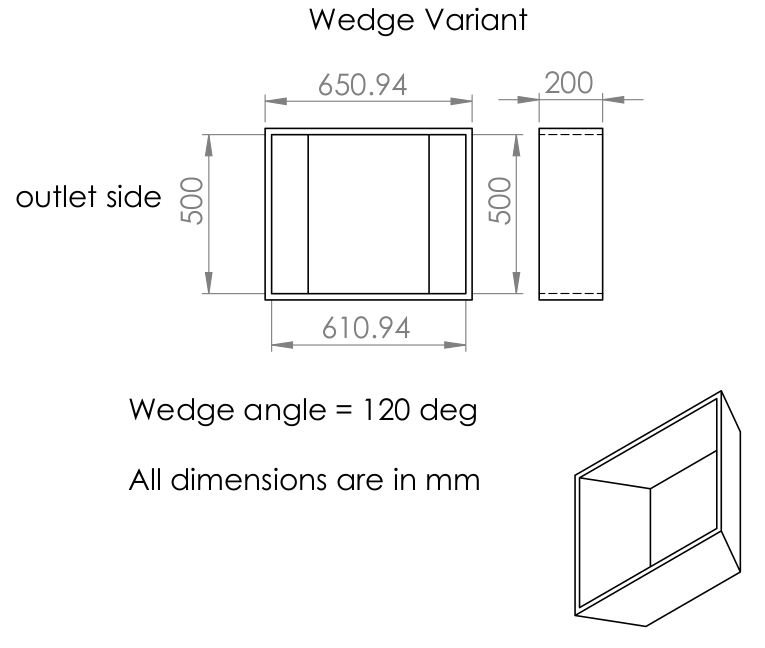
\includegraphics[width=80mm,scale=0.9]{w}
	\caption{example diagram}
	\label{fig:label10}
\end{figure}

Citing all the references: \cite{cite:1} \cite{cite:2} \cite{cite:3} \cite{cite:4} \cite{cite:5} \cite{cite:6} \cite{cite:7} \cite{cite:8} \cite{cite:9} \cite{cite:10} \cite{cite:11} \cite{cite:12} \cite{cite:13} \cite{cite:14} \cite{cite:15} \cite{cite:16} \cite{cite:17} \cite{cite:18} \cite{cite:19} \cite{cite:20} \cite{cite:21} \cite{cite:22} \cite{cite:23} \cite{cite:24} \cite{cite:25} \cite{cite:26} \cite{cite:27} \cite{cite:28} \cite{cite:29}



\end{document}